\documentclass{article}
\usepackage{amssymb}
\usepackage{tikz}
\usetikzlibrary{arrows,automata}
\newcounter{problem}
\newcounter{solution}

\newcommand\Problem{%
  \stepcounter{problem}%
  \textbf{\theproblem.}~%
  \setcounter{solution}{0}%
}

\newcommand\TheSolution{%
  \textbf{Solution \theproblem:}\\%
}

\newcommand\ASolution{%
  \stepcounter{solution}%
  \textbf{Solution \theproblem.\thesolution:}\\%
}
\parindent 0in
\parskip 1em
\begin{document}

\begin{center}
\fbox{\fbox{\parbox{4in}{\centering Assignment 4 by Lucas Karlsson}}}
\end{center}

\Problem Prove that $a^*(b+ab^*) = b + aa^*b^*.$

\TheSolution I read online about an algorithm to determine whether two RE are equal, one could construct NFA's
from both and then using these convert them into DFA's using subset construction and then minimize these using
a standard dfa minimization algorithm. And then compare these to see if they accpets the same language.

\textbf{Step 1.} Turning them into NFA's where \textbf{Q} = $a^*(b+ab^*)$ and \textbf{S} = $b+aa^*b^*$

\begin{center}
  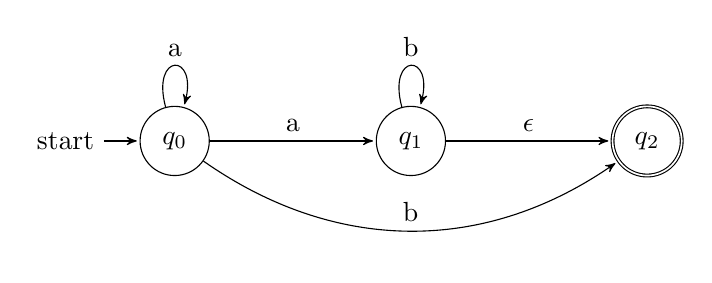
\begin{tikzpicture}[>=stealth',shorten >=1pt,auto,node distance=3cm]
    \node[initial,state]             (q0)                     {$q_0$};
    \node[state]           (q1) [right of=q0] {$q_1$};
    \node[accepting,state]                     (q2) [right of=q1] {$q_2$};

    \path[->] (q0) edge                node {a} (q1)
                   edge [loop above]   node {a} (q0)
                   edge [bend right=35] node {b} (q2)
              (q1) edge [loop above]   node {b} (q1)
                   edge                node {$\epsilon$} (q2);

  \end{tikzpicture}
\end{center}

\begin{center}
  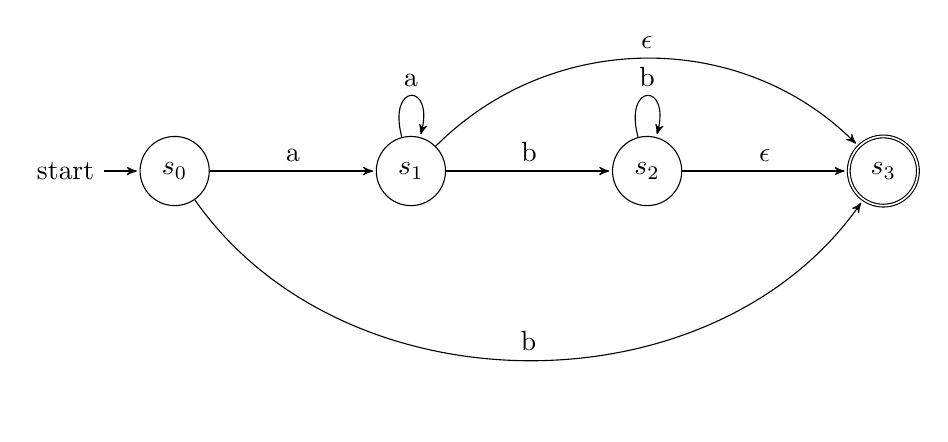
\begin{tikzpicture}[>=stealth',shorten >=1pt,auto,node distance=3cm]
    \node[initial,state]             (s0)               {$s_0$};
    \node[state]                     (s1) [right of=s0] {$s_1$};
    \node[state]                     (s2) [right of=s1] {$s_2$}; 
    \node[accepting,state]           (s3) [right of=s2] {$s_3$};

    \path[->] (s0) edge                 node {a} (s1)
                   edge [bend right=55] node {b} (s3)
              (s1) edge [loop above]    node {a} (s1)
                   edge                 node {b} (s2)
                   edge [bend left=45]  node {$\epsilon$} (s3)
              (s2) edge                 node {$\epsilon$} (s3)
                   edge [loop above]    node {b} (s2);

  \end{tikzpicture}
\end{center}

\newpage
\textbf{Step 2.} Now we can turn these NFA's into DFA's by removing the epsilon transitions and making
the states that had a epsilon transition into a accepting state a accepting state instead, doing this for 
\textbf{Q} and \textbf{S} will give us the result below. \textbf{Q} 

\begin{center}
  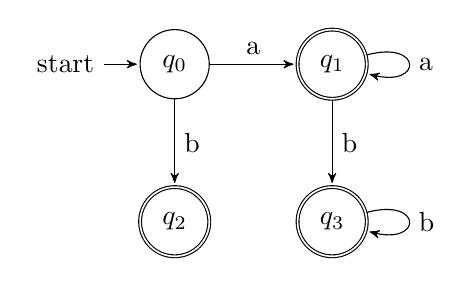
\begin{tikzpicture}[>=stealth',shorten >=1pt,auto,node distance=2cm]
    \node[initial,state]             (q0)               {$q_0$};
    \node[accepting,state]           (q1) [right of=q0] {$q_1$};
    \node[accepting,state]           (q2) [below of=q0] {$q_2$};
    \node[accepting,state]           (q3) [right of=q2] {$q_3$};

    \path[->] (q0) edge                 node {a} (q1)
                   edge                 node {b} (q2)
              (q1) edge [loop right]    node {a} (q2)
                   edge                 node {b} (q3)
              (q3) edge [loop right]    node {b} (q3);
  \end{tikzpicture}
\end{center}

\begin{center}
  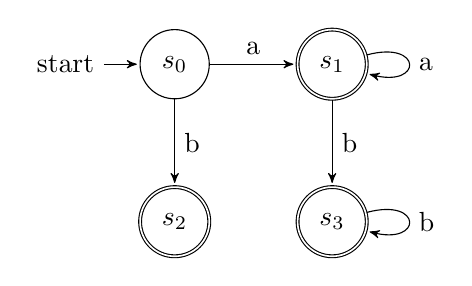
\begin{tikzpicture}[>=stealth',shorten >=1pt,auto,node distance=2cm]
    \node[initial,state]             (s0)               {$s_0$};
    \node[accepting,state]           (s1) [right of=s0] {$s_1$};
    \node[accepting,state]           (s2) [below of=s0] {$s_2$};
    \node[accepting,state]           (s3) [right of=s2] {$s_3$};

    \path[->] (s0) edge                 node {a} (s1)
                   edge                 node {b} (s2)
              (s1) edge [loop right]    node {a} (s2)
                   edge                 node {b} (s3)
              (s3) edge [loop right]    node {b} (s3);
  \end{tikzpicture}
\end{center}

\textbf{Step 3.} Well we can now see that the automatas are identical and will accept the same 
language and then by definition is equal to eachother.

\Problem Prove that every non regular language over an alphabet $\Sigma$ has an infinite
complement (with respect to $\Sigma^*$)

\TheSolution asd

\Problem Show that the language $\{w \in \{0,1,2\}^* \mid \#_0(w) + \#_1(w) =  \#_2(w)\}$ over the 
alphabet $\{0,1,2\}$ is not regular by using the pumping lemma for regular languages. Here $\#_a(w)$ 
is the number of occurences of a in w.

\TheSolution asd

\Problem Minimize the following DFA: (Do not just give the answer do a step by step)

\begin{table}[h!]
  \centering
  \begin{tabular}{c c c c}
    &&\textbf{0}&\textbf{1}\\ 
     \hfill $\to$ * & $s_0$ & $s_1$ & $s_3$\\
     \hfill         & $s_1$ & $s_4$ & $s_2$\\
     \hfill       * & $s_2$ & $s_1$ & $s_5$\\
     \hfill         & $s_3$ & $s_0$ & $s_4$\\
     \hfill         & $s_4$ & $s_4$ & $s_4$\\
     \hfill         & $s_5$ & $s_2$ & $s_4$\\[0.5ex]
  \end{tabular}
\end{table}

\TheSolution

\end{document}
